%%%%%%%%%%%%%%%%%%%%%%%%%%%%%%%%%%%%%%%%%%%%%%%%%%%%%%
% This is beamer setup. Not required for extraction. I personnaly like the default barebones style.
\documentclass{beamer}
\usepackage[utf8]{inputenc}
\usetheme{default}

%%%%%%%%%%%%%%%%%%%%%%%%%%%%%%%%%%%%%%%%%%%%%%%%%%%%%%
\usepackage{tikz}
\usepackage{bbm}
\usepackage{amsmath}
\usepackage{hyperref}

\usepackage{pdfpages} % import slides from Patricia

\newcommand\D{\mathrm{d}}
\newcommand\R{\mathbbm{R}}

\newcommand\Convolution{\ast}
\newcommand\Correlation{\star}

\newcommand\Reversed[1]{\overline{#1}}
\newcommand\Indicator[1]{\mathbbm{1}_{#1}}

\DeclareMathOperator{\nzd}{nzd}
\DeclareMathOperator{\IntervalLeft}{left}
\DeclareMathOperator{\IntervalRight}{right}
\DeclareMathOperator{\IntervalCenter}{center}

%%%%%%%%%%%%%%%%%%%%%%%%%%%%%%%%%%%%%%%%%%%%%%%%%%%%%%

\title{Calcul d'intégrales pour processus de Hawkes}
\author{François Gindraud \\ avec Anna Bonnet et Franck Picard}
\date{14 juin 2022}

\begin{document}

\maketitle

% Hawkes process, from slides of Patricia
{
    \setbeamercolor{background canvas}{bg=}
    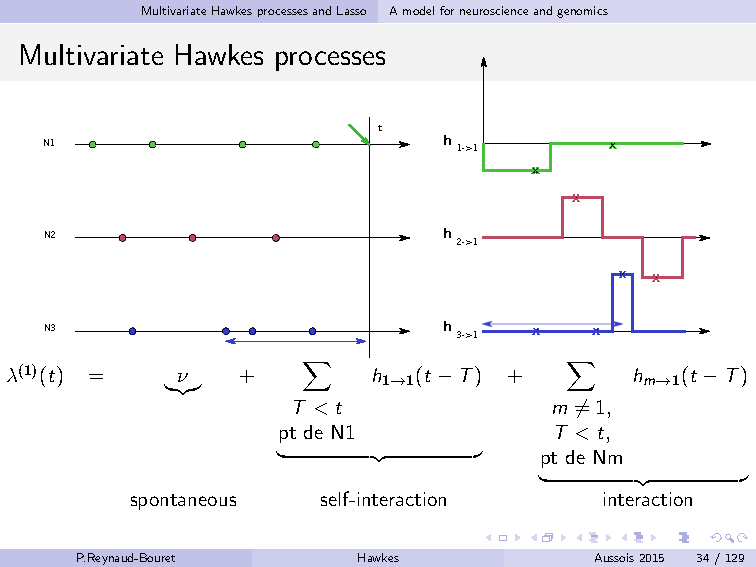
\includepdf{pg_0113.pdf}
}

\begin{frame}\frametitle{Function basis decomposition}
\[ h_{l \rightarrow m}(t - T) = \sum_{0 \le k < K} a_{k,l,m} \varphi_k(t - T) \]

\begin{columns}
    \begin{column}{0.4\textwidth}
        \textbf{Histograms}
        \small\[ \varphi_k = \frac{1}{\sqrt{\delta}} \mathbbm{1}_{]k\delta, (k+1)\delta]} \]
        \begin{center}\begin{tikzpicture}
            \draw[->] (-0.3,0) -- (3.5,0) node[right] {$x$};
            \draw[->] (0,-0.5) -- (0, 3.5);
            \node[below right] at (0, 0) {$0$};
            \draw[color=blue] (-0.3,0.3) node[left]{$\varphi_0$} -| (0,1) -| (1,0.3) -- (3.5,0.3);
            \draw[color=green] (-0.3,1.3) node[left]{$\varphi_1$} -| (1,2) -| (2,1.3) -- (3.5,1.3);
            \draw[color=red] (-0.3,2.3) node[left]{$\varphi_2$} -| (2,3) -| (3,2.3) -- (3.5,2.3);
        \end{tikzpicture}\end{center}
    \end{column}
    \begin{column}{0.6\textwidth}
        \textbf{Haar Wavelets}
        \small\[
            \varphi_{s,p} = \frac{\sqrt{2}^s}{\sqrt{\delta}} \left(
            \Indicator{ \left] \frac{2p \delta}{2^{s+1}}, \frac{(2p+1) \delta}{2^{s+1}} \right] } -
            \Indicator{ \left] \frac{(2p +1) \delta}{2^{s+1}}, \frac{(2p + 2) \delta}{2^{s+1}} \right] }
            \right)
        \]
        \small \[ 0 \le s < \text{Nscale} \qquad 0 \le p < 2^s \]
        \begin{center}\begin{tikzpicture}
            \draw[->] (-0.3,0) -- (4.5,0) node[right] {$x$};
            \draw[->] (0,-0.5) -- (0, 3.5);
            \node[below right] at (0, 0) {$0$};
            \draw[color=blue] (-0.3,0.5) node[left]{$\varphi_{0,0}$} -| (0,0.9) -| (2,0.1) -| (4,0.5) -- (4.5,0.5);
            \draw[color=green] (-0.3,1.5) node[left]{$\varphi_{1,0}$} -| (0,1.9) -| (1,1.1) -| (2,1.5) -- (4.5,1.5);
            \draw[color=red] (-0.3,2.5) node[left]{$\varphi_{1,1}$} -| (2,2.9) -| (3,2.1) -| (4,2.5) -- (4.5,2.5);
        \end{tikzpicture}\end{center}
    \end{column}
\end{columns}
\end{frame}

\end{document}